\chapter{Bevezetés} % User guide
\label{ch:bevezetes}

\section{A szükséges programok telepítése}

\subsection{A telepítő letöltése}
Code::blocks fejlesztői környezetre és c++ compiler-re (fordító program) lesz szükségünk, amelyeket egy csomagban le is tölthetünk és telepíthetünk a code::blocks oldaláról: \url{https://sourceforge.net/projects/codeblocks/}. Jelenleg erről a linkről windows-ra tölthetjük le a code::blocks-ot c++ fordító programmal együtt. 

Ez a legfrisebb code::blocks verzió, amely jelenleg szerepel az érettségi során használható programok listáján. (Ha érettségire készülünk, ellenőrizzük, hogy olyan verziót telepítsünk, amelyet majd használhatunk is az érettségi során, így véletlenül sem érhet meglepetés bennünket azon okból, hogy a mi verziónk eltérő attól, mint amit majd ott használhatunk.)

Amennyiben valami miatt ez a link nem működne, \url{https://www.codeblocks.org/downloads/} linken válasszuk ki a "Download the binary release" menüpontot.

\begin{figure}[H]
	\centering
	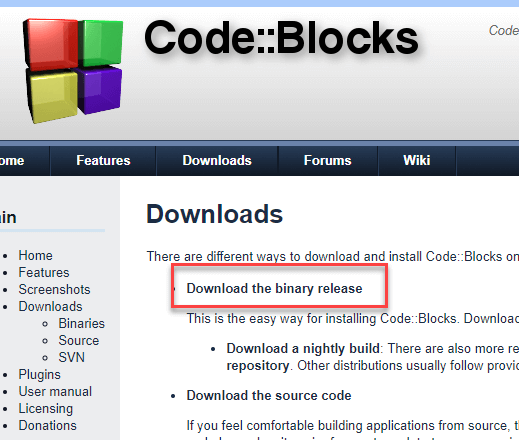
\includegraphics[width=0.5\linewidth]{images/bevezetes/choose}
	\caption{"Download the binary release"}
	\label{fig:choose}
\end{figure}

Ezt követően válasszuk ki a gcc compiler-rel való letöltését az intaller-nek.

\begin{figure}[H]
	\centering
	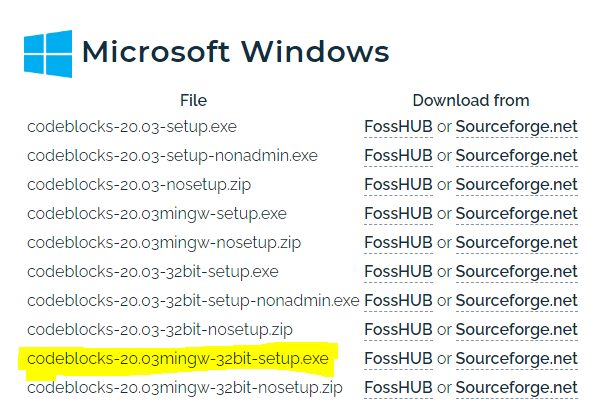
\includegraphics[width=0.8\linewidth]{images/bevezetes/download_installer}
	\caption{"Code::blocks telepítő gcc fordítóprogrammal való letöltése"}
	\label{fig:choose}
\end{figure}

\subsection{Telepítés}

A telepítő letöltését követően futtassuk azt. Mindent hagyjuk az alap beállításon, és navigáljunk keresztül a telepítőn. Esetleg a telepítés helyét módosíthatjuk, ha szeretnénk.

\subsection{A program üzembe helyezése}

A telepítést követően felajánlja számunkra a program elindítását a telepítő, javaslom, ezzel éljünk is. Az első indításnál ha minden jól megy, érzékeli is a program a fordító programot, amelyet a code::blocks-al együtt telepítettünk.

\begin{figure}[H]
	\centering
	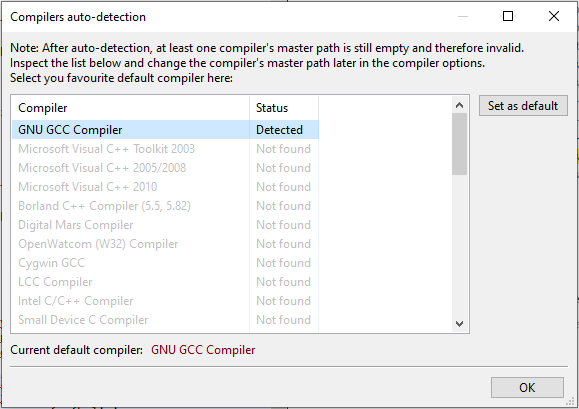
\includegraphics[width=1.0\linewidth]{images/bevezetes/set_compiler}
	\caption{Alapértelmezett fordítóprogram beállítása}
	\label{fig:choose}
\end{figure}

Válasszuk is ki a GNU GCC Compiler-t (ezt a fordítóprogramot telepítettük az imént a code::blocks-al együtt), menjünk a "Set as default"-ra (beállítás alapértelmezettként), majd kattintsuk az "OK"-ra.

Ezt követően megnyílik a program, és valószínűleg ismét egy felugró ablakba botlunk, amely arról érdeklődik, hogy szeretnénk-e bizonyos fájltípusok megnyitásához alapértelmezettként a code::blocks-ot rendelni. Ez azért lehet hasznos, mivel a későbbiekben egyszerűben dupla kattintással megnyithatjuk majd a projektjeinket, nem kell majd először a code::blocks-ot megnyitni, majd külön a programon belül kiböngészni a projektünket és úgy nyitni meg.

Én javaslom az alábbi menüpont kiválasztását.

\begin{figure}[H]
	\centering
	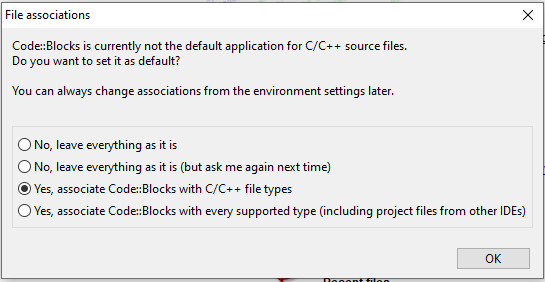
\includegraphics[width=0.7\linewidth]{images/bevezetes/associate_code_blocks}
	\caption{A c/c++ fájlok automatikusan code::blocks-al nyíljanak meg}
	\label{fig:choose}
\end{figure}

Ha minden igaz, ezt követően már használhatjuk is kisebb c++ projektek elkészítéséhez fejlesztői környezetünket, azonban ajánlom leellenőrizni a fordítóprogram beállításait: gyakori hiba kezdetben a code::blocks-nál, hogy nem találja azt, emiatt nem tudja lefordítani a forráskódjainkat.

Válasszuk ki a fejlécben a "Settings"-t majd a legördülő menüben a "Compiler"-t.


\begin{figure}[H]
	\centering
	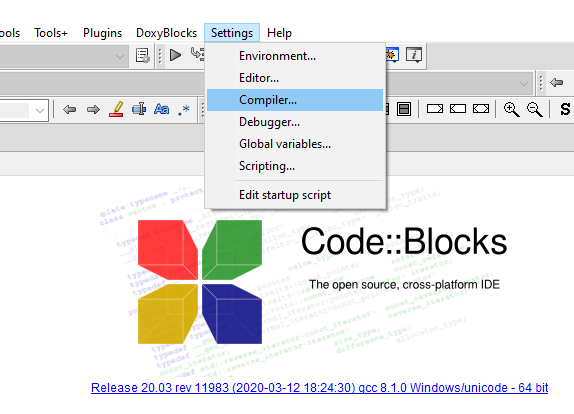
\includegraphics[width=0.7\linewidth]{images/bevezetes/check_compiler_01}
	\caption{A fordítóprogram beállításainak ellenőrzése}
	\label{fig:choose}
\end{figure}

Ezt követően a felugró ablak felső részében elhelyezkedő menüpontok közül válasszuk ki a "Toolchain executables"-t. Itt a fordítóprogram helyének kell lennie. Amennyiben minden jól ment, itt már szerepel egy elérési útvonal, ha a telepítés helyét a default-on hagytuk, akkor pontosan oda hivatkozik, ahova az a képen is látható.

\begin{figure}[H]
	\centering
	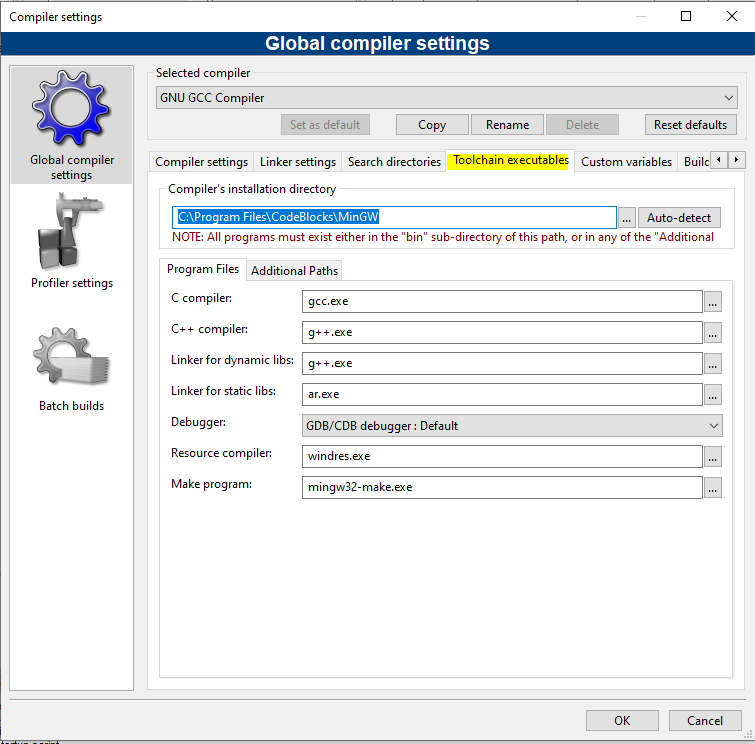
\includegraphics[width=1.0\linewidth]{images/bevezetes/check_compiler_02}
	\caption{A fordítóprogram helyének ellenőrzése}
	\label{fig:choose}
\end{figure}

Ha szeretnénk beállítani, hogy a c++ mely standard-ját szeretnénk használni (bizonyos években "frissítik" a programozási nyelveket is, akár a programokat, de jó esetben az újítások után is használhatóak lesznek a régebbi megoldások is), azt szintén itt, a "Compiler settings" almenüben tehetjük meg.

\begin{figure}[H]
	\centering
	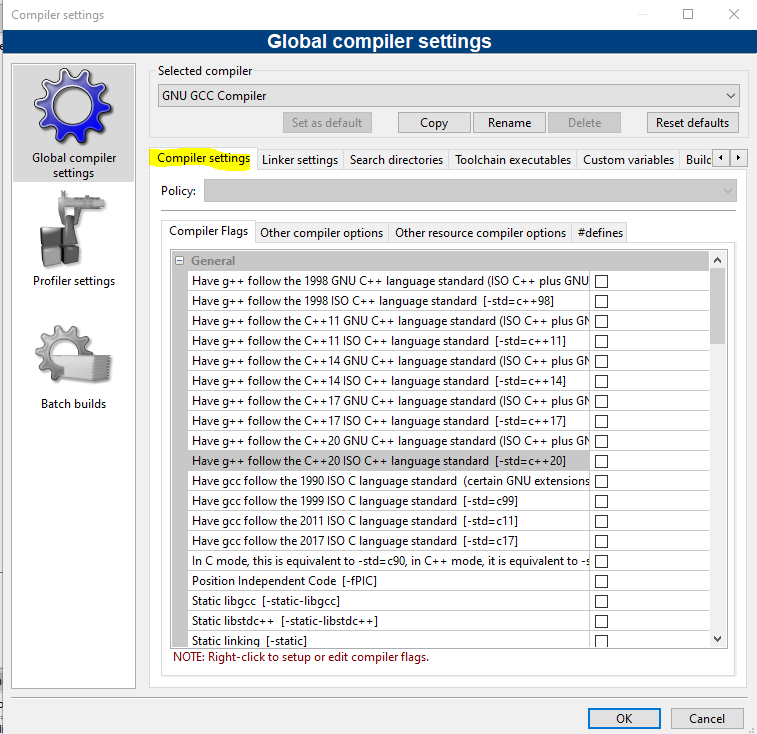
\includegraphics[width=1.0\linewidth]{images/bevezetes/check_compiler_03}
	\caption{A fordítóprogram standard-jának ellenőrzése}
	\label{fig:choose}
\end{figure}

Ahogyan azt a képen is láthatjuk, a 2020-as standard a legfrissebb jelenleg. Jómagam azt javaslom, hogy amennyiben érettségire készülünk, válasszuk a legfrissebb olyan standard-et, amelyet ott is használhatunk, amennyiben nem, válasszuk a legfrissebbet.

\section{Alapvető fogalmak}

Ebben a részben olyan fogalmak jelentését fogjuk tisztázni, amelyek a legtöbbször előfordulnak, ha programozásról van szó, esetleg a korábbiakban is említésre kerültek már.

\paragraph{Programozási nyelv}
A programozási nyelv célja, hogy olyan módon írhassuk le programok működését, amely emberek számára is olvasható, megérthető, jól strukturált, és egyértelmű. Azonban ezek a számítógép számára alapból nem értelmezhetőek, ezért szükséges fordító program (compiler) használata, amely gépi kódra, azaz a számítógép számára értelmezhető, futtatható formába alakítja azt át. A programozási nyelvek között vannak ún. alacsonyabb és magasabb szintűek. Az alacsonyabb szintűek közelebb állnak a gépi kódhoz, a magasabb szintűek pedig távolabb, ezek segítségével álltalában bonyolultbb logikájú, stukturáltabb programokat írhatunk. Ilyen magasabb szintű programozási nyelv többek között a c++ is. Programozóként nem nagyon fogunk alacsony szintű programozási nyelvekkel találkozni. Bővebben lásd: \url{https://hu.wikipedia.org/wiki/Programoz%C3%A1si_nyelv}.

\paragraph{Fordítóprogram} A fordítóprogram olyan program, amely valamely programozási nyelvben írt programot gépi kódra, számítógép által értelmezhető, futtatható formára alakít át. Bővebben lásd.: \url{https://hu.wikipedia.org/wiki/Ford%C3%ADt%C3%B3program}.

\paragraph{Fejlesztői környezet}
Olyan program (ez lehet bármi egyéb is, de az egyszerűség kedvéért gondoljunk most programra), amely funkcióival segíti a programozó dolgát: például megjeleníti a programkódot, ily módon ez lehet egy egyszerű jegyzettömb is. Kicsit bonyolultabb fejlesztői környezet például a code::blocks is, bár ez azért jóval több funkciót kínál, mint egy egyszerű jegyzettömb. Például segítségével lefordíthatjuk és futtathatjuk is programunkat. A programkódot sem egyszerűen, hanem ún. "syntax highlight"-al jeleníti meg. Ez egyszerűen annyit takar, hogy bizonyos kulcsszavakat különböző színűre színez, így átláthatóbb a kód. Bővebben lásd.: \url{https://hu.wikipedia.org/wiki/Fejleszt%C5%91i_k%C3%B6rnyezet}.

\paragraph{Forrásfájl}
Olyan fájl, amely a program kódját tartalmazza. Nagyobb programok álltalában több forrásfájlból állnak.

\paragraph{Forráskód} A program még le nem fordított állapotban lévő kódja, amelyet a forrásfájlok tartalmaznak (nagyobb programok esetén ez több forrásfájlból áll). Ez nem futtható, csak fordítás után. (Amelyet a fordítóprogram, angol kifejezéssel compiler [kompájler] végez el.) Ha egy program forráskódja a rendelkezésünkre áll, akkor azt továbbfejleszthetjük, esetleg funkcióit módosíthatjuk segítségével. Ezt a bináris (gépi kód) verzión nem tehetjük meg. Ezért tulajdonképpen ez a program lelke.

\section{Az első programom}
